% Template for Cogsci submission with R Markdown

% Stuff changed from original Markdown PLOS Template
\documentclass[10pt, letterpaper]{article}

\usepackage{cogsci}
\usepackage{pslatex}
\usepackage{float}
\usepackage{caption}

% amsmath package, useful for mathematical formulas
\usepackage{amsmath}

% amssymb package, useful for mathematical symbols
\usepackage{amssymb}

% hyperref package, useful for hyperlinks
\usepackage{hyperref}

% graphicx package, useful for including eps and pdf graphics
% include graphics with the command \includegraphics
\usepackage{graphicx}

% Sweave(-like)
\usepackage{fancyvrb}
\DefineVerbatimEnvironment{Sinput}{Verbatim}{fontshape=sl}
\DefineVerbatimEnvironment{Soutput}{Verbatim}{}
\DefineVerbatimEnvironment{Scode}{Verbatim}{fontshape=sl}
\newenvironment{Schunk}{}{}
\DefineVerbatimEnvironment{Code}{Verbatim}{}
\DefineVerbatimEnvironment{CodeInput}{Verbatim}{fontshape=sl}
\DefineVerbatimEnvironment{CodeOutput}{Verbatim}{}
\newenvironment{CodeChunk}{}{}

% cite package, to clean up citations in the main text. Do not remove.
\usepackage{cite}

\usepackage{color}

% Use doublespacing - comment out for single spacing
%\usepackage{setspace}
%\doublespacing


% % Text layout
% \topmargin 0.0cm
% \oddsidemargin 0.5cm
% \evensidemargin 0.5cm
% \textwidth 16cm
% \textheight 21cm

\title{Sources of knowledge in children's acquisition of the successor function}


\author{{\large \bf Rose M. Schneider, Kaiqi Guo} and {\large \bf David Barner} \\ \{roschnei, kaguo, barner \} @ucsd.edu \\ Department of Psychology \\ University of California, San Diego}

\begin{document}

\maketitle

\begin{abstract}
Through understanding the successor function, i.e.~for any natural
number n, its successor is n+1, we can gain the insight that the natural
numbers are infinite. Recent work has suggested acquisition of this
logical property is more protracted than previously thought, with a
fully generalized understanding of the successor function not apparent
until 5.5 to 6 years of age. While such work links successor knowledge
with counting mastery, the exact processes underlying this developmental
transition remain unknown. Here, we examined two hypothesized
mechanisms: (1) productive counting knowledge, or mastery of the
recursive process through which number words are generated, and (2)
formally trained arithmetic, specifically the `+1' operation. We tested
the relationship between successor knowledge, productive counting, and
arithmetic proficiency in 140 3.5 to 6 year-olds. We found that while
both productive counting and arithmetic mastery predicted successor
knowledge, mean arithmetic performance was significantly lower for all
children, even those at ceiling in implementing the successor function
This surprising dissociation suggests children do not draw upon the `+1'
operation in acquiring the successor function. Rather, these findings
are more consistent with the hypothesis that this knowledge is acquired
through productive counting, and the recognition that numbers are
recursively generated through an implementation of the successor
function.

\textbf{Keywords:}
Add your choice of indexing terms or keywords; kindly use a semi-colon;
between each term.
\end{abstract}

\section{Introduction}\label{introduction}

One of our most profound achievements as learners is the ability to
extract limitlessly productive rules from limited data. While this
capacity makes us prodigious learners in general, one of its most
powerful applications is in the domain of number. Although linguistic
number input and expression are undoubtedly finite, we nevertheless come
to know the natural numbers to be infinite; for every number, its
successor can be obtained by simply adding `1.' Further, we understand
that this successor function can be endlessly implemented due to the
recursive nature of symbolic number. How does such an understanding
arise? In this work, we explored two hypothesized causal mechanisms
(productive counting knowledge and formally trained arithmetic) by which
children might acquire the successor function, a critical component in
the logical framework of natural number.

Early in numerical development, children do not treat number as a
productive form of representation. Although they may be able to recite
the count list up to about 10 (Fuson 1988), they do not acquire the
meanings of these numerals until much later, with one, two, and three
effortfully acquired over the course of about 12 months (Wynn, 1992).
Around the time that children acquire the meaning of four, however, they
suddenly seem to understand the relationship between their memorized
count list and cardinality, referred to as the Cardinal Principle (CP).

Even after children acquire the CP, however, they may not yet understand
that numbers are generated through a recursive process. Recent work has
found evidence that children do not understand the successor function as
a truly generalized property of natural number until several years after
acquisition of the CP. While many children who have acquired the CP
(CP-knowers) can implement the successor function for small numbers,
such as 4 or 5 (Sarnecka \& Carey, 2008), their ability to do so for any
number is mediated by their counting proficiency (Davidson, Eng, \&
Barner, 2012; Cheung, Rubenson, \& Barner, 2017). In this work, only
children who demonstrate mastery of the count list are able to apply the
successor function to any number queried. These results indicate that
counting proficiency, rather than CP-knowledge, is implicated in
acquisition of this logical property.

This observed correlation with counting mastery suggests two potential
paths by which children might acquire the successor function. The first,
which we refer to as productive counting knowledge, is that as children
come to understand the recursive nature of number, they notice that the
next number generated via that process is always done so by the addition
of `1,' or an implementation of the successor function (Cheung et al.,
2017). This hypothesis would therefore predict that children who
specifically demonstrate knowledge of recursion are more likely to have
acquired the successor function.

The second hypothesized mechanism is that children learn the successor
function through explicit instruction, rather than an induction made
over the count list. As children learn formal arithmetic operations,
such as 4+1=5 and 5+1=6, it is possible that they hypothesize the `+1'
rule to hold true for any number. On this account, we would expect to
find that children's successor function knowledge is significantly
related to mastery of these rote-learned `math facts.' In the present
work, we tested these two potential paths to successor function
acquisition in 140 3.5- to 6-year-old CP-knowers (3.58 -- 5.98, Mage =
4.9, SDage = 0.61, ). We used a modified version of the Unit Task
(Sarnecka \& Carey, 2008) to test children's successor knowledge. In
this task, an experimenter placed some number of fish on a board, and
said, ``Look! There are N fish in the pond.'' The experimenter then
covered these fish with a lilypad, and placed one additional fish next
to the lilypad, saying ``Look! Are there N+1 or N+2 fish now?'' Children
received 16 trials, with N ranging from 6 to 95.

\section{Method}\label{method}

\subsection{Participants}\label{participants}

We recruited 140 children between the ages of 3;6 and 5;11 (\emph{M} =
4.89, \emph{SD} = 0.61) out of a planned sample of 150.

\subsection{Stimuli and Design}\label{stimuli-and-design}

\subsection{Procedure}\label{procedure}

First level headings should be in 12 point , initial caps, bold and
centered. Leave one line space above the heading and
1/4\textasciitilde{}line space below the heading.

\section{Results}\label{results}

Second level headings should be 11 point , initial caps, bold, and flush
left. Leave one line space above the heading and 1/4\textasciitilde{}
line space below the heading.

\section{Discussion}\label{discussion}

Third-level headings should be 10 point , initial caps, bold, and flush
left. Leave one line space above the heading, but no space after the
heading.

\section{Formalities, Footnotes, and
Floats}\label{formalities-footnotes-and-floats}

Use standard APA citation format. Citations within the text should
include the author's last name and year. If the authors' names are
included in the sentence, place only the year in parentheses, as in
(1972), but otherwise place the entire reference in parentheses with the
authors and year separated by a comma (Newell \& Simon, 1972). List
multiple references alphabetically and separate them by semicolons
(Chalnick \& Billman, 1988; Newell \& Simon, 1972). Use the et. al.
construction only after listing all the authors to a publication in an
earlier reference and for citations with four or more authors.

For more information on citations in RMarkdown, see
\textbf{\href{http://rmarkdown.rstudio.com/authoring_bibliographies_and_citations.html\#citations}{here}.}

\subsection{Footnotes}\label{footnotes}

Indicate footnotes with a number\footnote{Sample of the first
footnote.} in the text. Place the footnotes in 9 point type at the
bottom of the page on which they appear. Precede the footnote with a
horizontal rule.\footnote{Sample of the second footnote.} You can also
use markdown formatting to include footnotes using this
syntax.\footnote{Sample of a markdown footnote.}

\subsection{Figures}\label{figures}

All artwork must be very dark for purposes of reproduction and should
not be hand drawn. Number figures sequentially, placing the figure
number and caption, in 10 point, after the figure with one line space
above the caption and one line space below it. If necessary, leave extra
white space at the bottom of the page to avoid splitting the figure and
figure caption. You may float figures to the top or bottom of a column,
or set wide figures across both columns.

\subsection{Two-column images}\label{two-column-images}

You can read local images using png package for example and plot it like
a regular plot using grid.raster from the grid package. With this method
you have full control of the size of your image. \textbf{Note: Image
must be in .png file format for the readPNG function to work.}

You might want to display a wide figure across both columns. To do this,
you change the \texttt{fig.env} chunk option to \texttt{figure*}. To
align the image in the center of the page, set \texttt{fig.align} option
to \texttt{center}. To format the width of your caption text, you set
the \texttt{num.cols.cap} option to \texttt{2}.

\begin{CodeChunk}
\begin{figure*}[h]

{\centering 
\includegraphics{figs/2-col-image-1} 

}

\caption[This image spans both columns]{This image spans both columns. And the caption text is limited to 0.8 of the width of the document.}\label{fig:2-col-image}
\end{figure*}
\end{CodeChunk}

\subsection{One-column images}\label{one-column-images}

Single column is the default option, but if you want set it explicitly,
set \texttt{fig.env} to \texttt{figure}. Notice that the
\texttt{num.cols} option for the caption width is set to \texttt{1}.

\begin{CodeChunk}
\begin{figure}[H]

{\centering 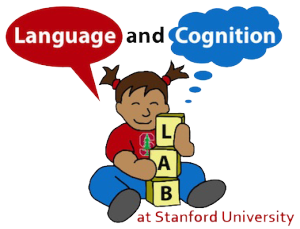
\includegraphics{figs/image-1} 

}

\caption[One column image]{One column image.}\label{fig:image}
\end{figure}
\end{CodeChunk}

\subsection{R Plots}\label{r-plots}

You can use R chunks directly to plot graphs. And you can use latex
floats in the fig.pos chunk option to have more control over the
location of your plot on the page. For more information on latex
placement specifiers see
\textbf{\href{https://en.wikibooks.org/wiki/LaTeX/Floats,_Figures_and_Captions}{here}}

\begin{CodeChunk}
\begin{figure}[H]

{\centering 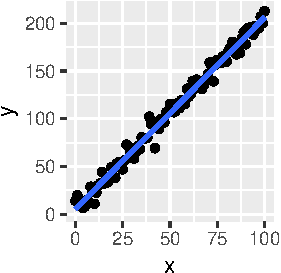
\includegraphics{figs/plot-1} 

}

\caption[R plot]{R plot}\label{fig:plot}
\end{figure}
\end{CodeChunk}

\subsection{Tables}\label{tables}

Number tables consecutively; place the table number and title (in 10
point) above the table with one line space above the caption and one
line space below it, as in Table 1. You may float tables to the top or
bottom of a column, set wide tables across both columns.

You can use the xtable function in the xtable package.

\begin{table}[H]
\centering
\begin{tabular}{rrrrr}
  \hline
 & Estimate & Std. Error & t value & Pr($>$$|$t$|$) \\ 
  \hline
(Intercept) & -0.03 & 0.09 & -0.3 & 0.78 \\ 
  x & 2.08 & 0.09 & 23.4 & 0.00 \\ 
   \hline
\end{tabular}
\caption{This table prints across one column.} 
\end{table}

\section{Acknowledgements}\label{acknowledgements}

Place acknowledgments (including funding information) in a section at
the end of the paper.

\section{References}\label{references}

\setlength{\parindent}{-0.1in} \setlength{\leftskip}{0.125in} \noindent

\hypertarget{refs}{}
\hypertarget{ref-ChalnickBillman1988a}{}
Chalnick, A., \& Billman, D. (1988). Unsupervised learning of
correlational structure. In \emph{Proceedings of the tenth annual
conference of the cognitive science society} (pp. 510--516). Hillsdale,
NJ: Lawrence Erlbaum Associates.

\hypertarget{ref-NewellSimon1972a}{}
Newell, A., \& Simon, H. A. (1972). \emph{Human problem solving}.
Englewood Cliffs, NJ: Prentice-Hall.

\end{document}
